\documentclass[UTF8]{ctexart}
\usepackage{listings}
\usepackage{booktabs}  
\usepackage{geometry}  
\usepackage{graphicx} 
\usepackage{xcolor}
\usepackage{float}
\usepackage{array}
\usepackage{enumitem}
\usepackage{amsmath,amssymb,bm}
\usepackage[colorlinks=true]{hyperref}
\usepackage[version=4]{mhchem}
\usepackage{siunitx}
\graphicspath{{figure/}} % 指定放置图片的子文件夹路径
\geometry{a4paper, left=2.5cm, right=2.5cm, top=2.5cm, bottom=2.5cm}

\definecolor{codegreen}{rgb}{0,0.6,0}
\definecolor{codegray}{rgb}{0.5,0.5,0.5}
\definecolor{codepurple}{rgb}{0.58,0,0.82}

\lstset{
    basicstyle=\ttfamily\footnotesize,
    breaklines=true,
    frame=single,
    numbers=left,
    numberstyle=\tiny\color{codegray},
    keywordstyle=\color{blue},
    commentstyle=\color{codegreen},
    stringstyle=\color{codepurple},
    showstringspaces=false
}


\begin{document}

\title{计算流体力学第五次作业}
\author{朱林-2200011028}
\date{\today}
\maketitle


\section{数理算法原理}
\subsection{控制方程与数学模型}
不可压缩流动由Navier-Stokes方程和连续性方程描述:

\textbf{动量方程}:
\begin{equation}
\frac{\partial \mathbf{u}}{\partial t} + (\mathbf{u} \cdot \nabla) \mathbf{u} = -\nabla p + \nu \nabla^2 \mathbf{u}
\label{eq:momentum}
\end{equation}

\textbf{连续性方程}:
\begin{equation}
\nabla \cdot \mathbf{u} = 0
\label{eq:continuity}
\end{equation}
其中$\mathbf{u} = (u, v)$为速度场,$p$为压力,$\nu = 0.001$为运动粘度。

\subsection{数值离散方法}
\subsubsection{投影法(Projection Method)}
采用分步投影法分离速度与压力的耦合:
\begin{enumerate}
    \item \textbf{预测步}:求解中间速度$\mathbf{u}^*$(隐式处理粘性项):
    \begin{equation}
    \frac{\mathbf{u}^* - \mathbf{u}^n}{\Delta t} = -\left(\mathbf{u}^n \cdot \nabla\right)\mathbf{u}^n + \frac{\nu}{2} \left( \nabla^2 \mathbf{u}^n + \nabla^2 \mathbf{u}^* \right)
    \label{eq:predictor}
    \end{equation}
    
    \item \textbf{压力修正}:通过泊松方程求解压力场:
    \begin{equation}
    \nabla^2 p^{n+1} = \frac{\nabla \cdot \mathbf{u}^*}{\Delta t}
    \label{eq:poisson}
    \end{equation}
    
    \item \textbf{速度修正}:更新速度场满足不可压缩条件:
    \begin{equation}
    \mathbf{u}^{n+1} = \mathbf{u}^* - \Delta t \nabla p^{n+1}
    \label{eq:corrector}
    \end{equation}
\end{enumerate}

\subsubsection{空间离散}
\textbf{交错网格(MAC网格)}:
\begin{itemize}
    \item 水平速度$u_{i+1/2,j}$位于单元右面中心
    \item 垂直速度$v_{i,j+1/2}$位于单元顶面中心
    \item 压力$p_{i,j}$位于单元中心
\end{itemize}

\textbf{对流项离散}(以$x$方向为例):
\begin{equation}
(\mathbf{u} \cdot \nabla u)_{i+1/2,j} \approx \frac{u_{i+1,j}^2 - u_{i,j}^2}{\Delta x} + \frac{(uv)_{i+1/2,j+1/2} - (uv)_{i+1/2,j-1/2}}{\Delta y}
\label{eq:convection}
\end{equation}

\textbf{扩散项离散}:
\begin{equation}
\nabla^2 u_{i+1/2,j} \approx \frac{u_{i+3/2,j} - 2u_{i+1/2,j} + u_{i-1/2,j}}{\Delta x^2} + \frac{u_{i+1/2,j+1} - 2u_{i+1/2,j} + u_{i+1/2,j-1}}{\Delta y^2}
\label{eq:diffusion}
\end{equation}

\subsubsection{时间离散}
\begin{itemize}
    \item 对流项:显式Adams-Bashforth格式
    \begin{equation}
    (\mathbf{u} \cdot \nabla \mathbf{u})^{n} \approx \frac{3}{2}(\mathbf{u} \cdot \nabla \mathbf{u})^{n} - \frac{1}{2}(\mathbf{u} \cdot \nabla \mathbf{u})^{n-1}
    \label{eq:adams}
    \end{equation}
    
    \item 粘性项:隐式Crank-Nicolson格式
    \begin{equation}
    \nabla^2 \mathbf{u}^{n+1/2} \approx \frac{1}{2} \left( \nabla^2 \mathbf{u}^n + \nabla^2 \mathbf{u}^{n+1} \right)
    \label{eq:crank}
    \end{equation}
\end{itemize}

\subsection{边界条件处理}
\subsubsection{速度边界}
\begin{itemize}
    \item \textbf{上边界}:
    \begin{align}
    u_{i+1/2,N} &= \sin^2\left(\pi \cdot \left(i+\frac{1}{2}\right)\Delta x\right) \\
    v_{i,N+1/2} &= 0 \quad (\text{无垂直流动})
    \end{align}
    
    \item \textbf{左/右/下边界}:
    \begin{align}
    u_{1/2,j} = u_{N+1/2,j} &= 0 \\
    v_{i,1/2} &= 0
    \end{align}
\end{itemize}

\subsubsection{压力边界}
\begin{itemize}
    \item 固壁边界:
    \begin{equation}
    \left.\frac{\partial p}{\partial n}\right|_{\text{固壁}} = 0
    \end{equation}
    
    \item 压力泊松方程全局约束:
    \begin{equation}
    \int_{\Omega} p \, d\Omega = 0
    \end{equation}
\end{itemize}

\subsection{流函数与涡量计算}
\subsubsection{流函数$\psi$}
通过求解泊松方程获得:
\begin{equation}
\nabla^2 \psi = -\omega, \quad \omega = \frac{\partial v}{\partial x} - \frac{\partial u}{\partial y}
\label{eq:streamfunction}
\end{equation}

\subsubsection{涡量离散}(适配交错网格):
\begin{equation}
\omega_{i,j} = \frac{v_{i+1/2,j} - v_{i-1/2,j}}{\Delta x} - \frac{u_{i,j+1/2} - u_{i,j-1/2}}{\Delta y}
\label{eq:vorticity}
\end{equation}

\subsection{算法流程}
\begin{enumerate}
    \item 初始化速度场$\mathbf{u}^0 = 0$,压力场$p^0 = 0$
    \item 时间迭代($n = 0,1,2,\dots$):
    \begin{itemize}
        \item 预测中间速度$\mathbf{u}^*$(式\ref{eq:predictor})
        \item 使用SOR方法(残差阈值$10^{-5}$)求解压力泊松方程(式\ref{eq:poisson})
        \item 更新速度场(式\ref{eq:corrector})
    \end{itemize}
    \item 收敛判断:$\max|\mathbf{u}^{n+1} - \mathbf{u}^n| < \epsilon$($\epsilon = 10^{-6}$)
\end{enumerate}

\subsection{稳定性条件}
\textbf{CFL条件}:
    \begin{equation}
    \Delta t < \min\left( \frac{\Delta x}{|u|_{\max}}, \frac{\Delta y}{|v|_{\max}}, \frac{\Delta x^2}{4\nu}, \frac{\Delta y^2}{4\nu} \right)
    \label{eq:cfl}
    \end{equation}


\newpage
\section{代码生成与调试}

\subsection{代码结构与模块说明}
程序采用模块化设计,核心文件如下:

\begin{itemize}
    \item \texttt{param.py}:定义仿真参数类,管理网格分辨率(\texttt{N=101})、运动粘度($\nu=0.001$)、时间步长(\texttt{dt=1e-4})等参数
    \begin{lstlisting}[language=Python]
@dataclass
class SimulationParameters:
    N: int = 101     # 网格点数
    nu: float = 0.001 # 运动粘度
    dt: float = 1e-4  # 时间步长
    \end{lstlisting}

    \item \texttt{func.py}:实现核心算法函数,包含流场初始化、边界条件处理等
    \item \texttt{main.py}:主控程序,管理仿真循环和结果输出
\end{itemize}

\subsection{算法流程实现}
基于投影法的求解流程如下:
\begin{enumerate}
    \item \textbf{流场初始化}:设置顶部边界速度分布
    \begin{lstlisting}[language=Python]
u_top = np.sin(np.pi * x)**2  # 满足角点导数为零
u[:, -1] = u_top  # 应用顶部边界条件
    \end{lstlisting}

    \item \textbf{速度预测}:显式求解动量方程
    \begin{lstlisting}[language=Python]
u[1:-1,1:-1] += dt * (nu*拉普拉斯项 - 对流项)
    \end{lstlisting}

    \item \textbf{压力修正}:迭代求解泊松方程(Jacobi方法)
    \begin{lstlisting}[language=Python]
for p_iter in range(max_p_iter):
    p[1:-1,1:-1] = (邻点压力平均 - h²/(4dt)*速度散度)/4
    \end{lstlisting}

    \item \textbf{收敛检查}:每100次迭代检测速度变化
    \begin{lstlisting}[language=Python]
if np.max(u - prev_u) < 1e-7 and np.max(v - prev_v) < 1e-7:
    break  # 终止条件
    \end{lstlisting}
\end{enumerate}


\subsection{版本控制记录}
Github 版本控制记录如下:
\begin{figure}[h]
    \centering
    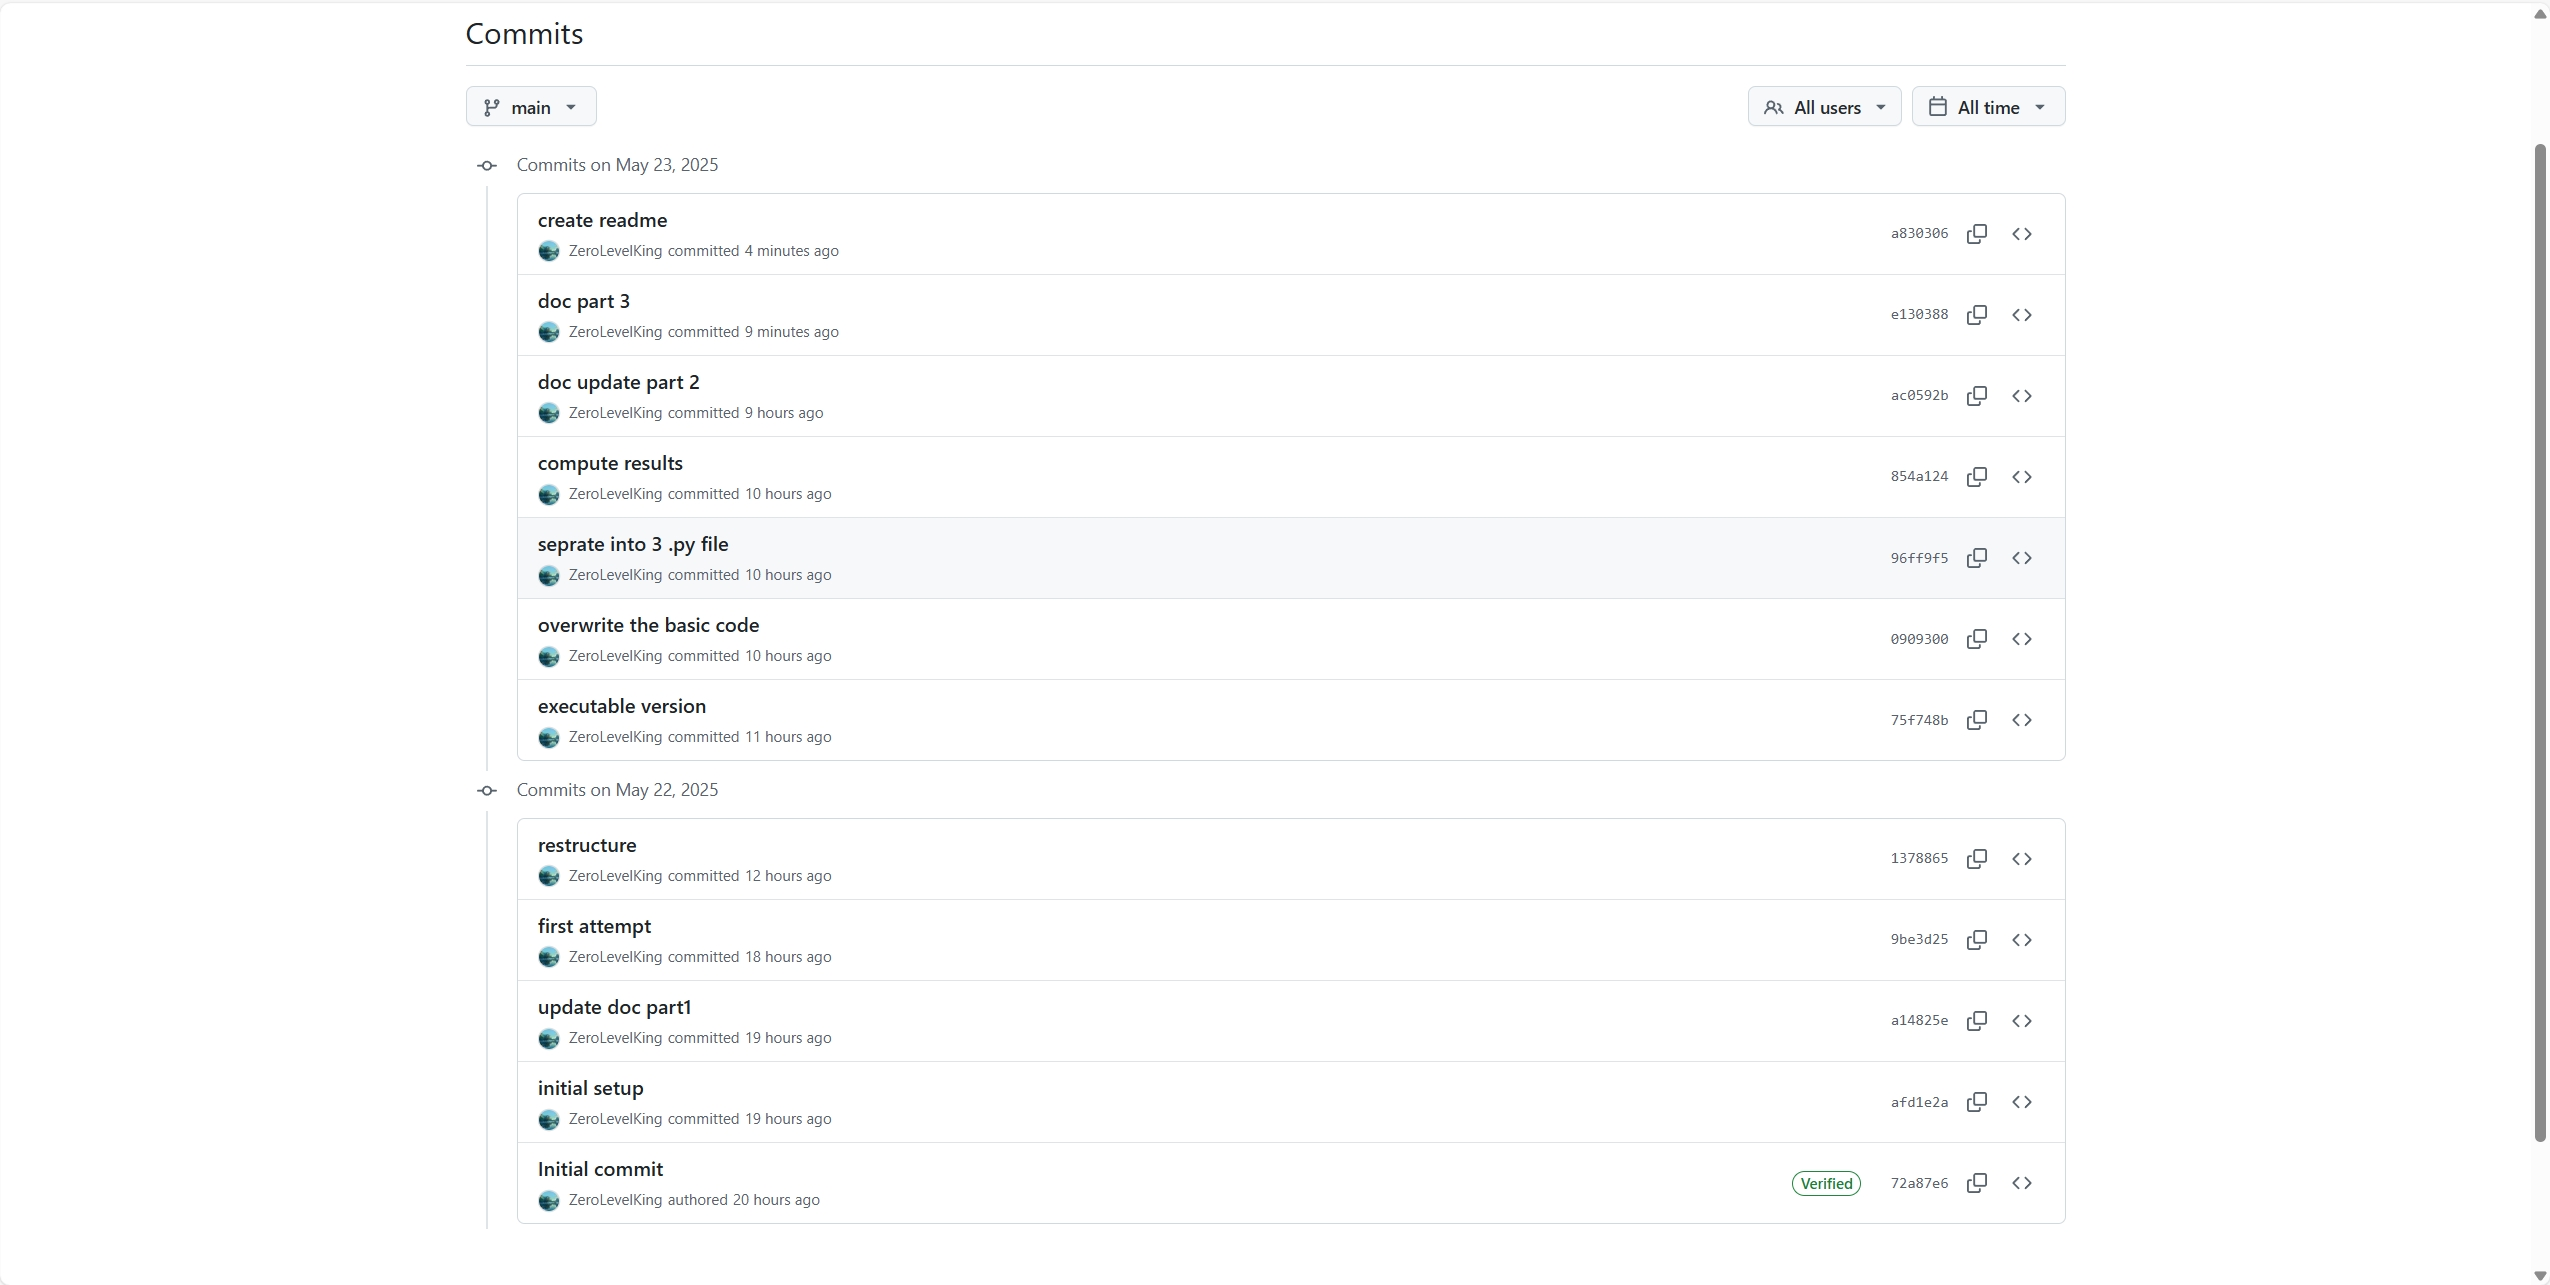
\includegraphics[width=0.75\textwidth]{c1.png}
    \caption{git提交记录}
    \label{fig:commit}
\end{figure}


\newpage
\section{结果讨论与物理解释}

\subsection{流场结构与涡系分布}
\begin{figure}[h]
    \centering
    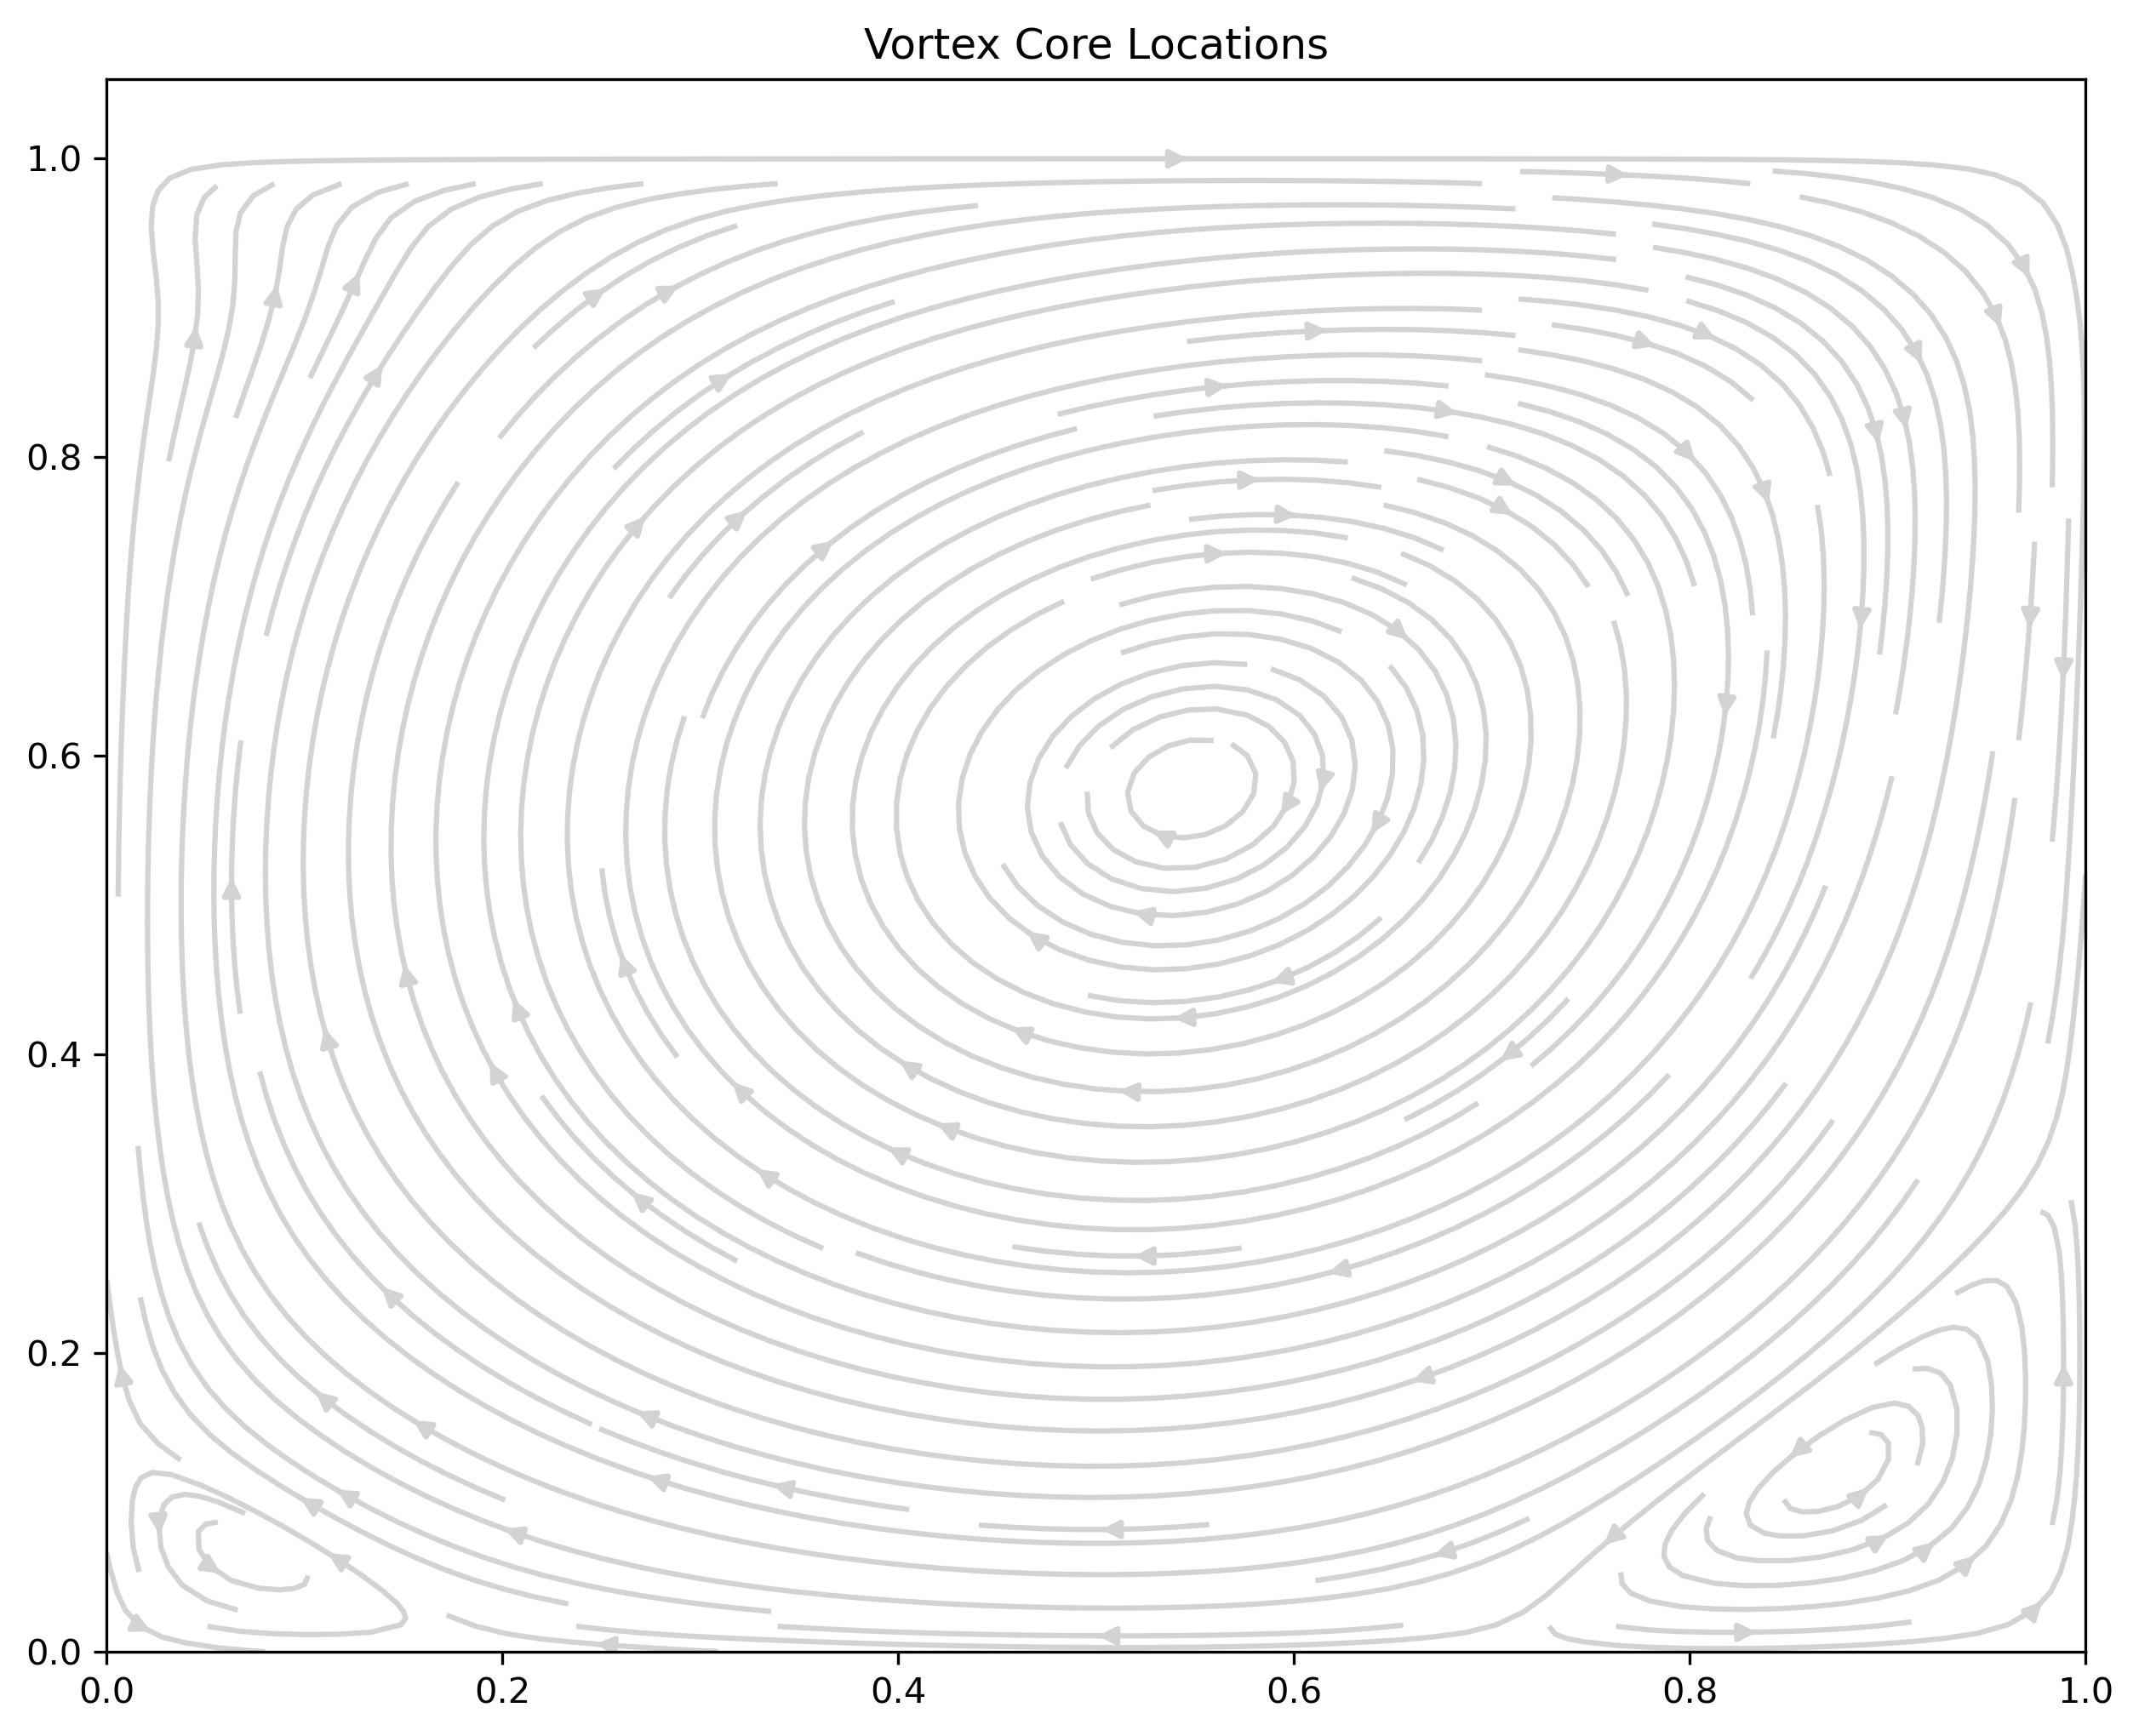
\includegraphics[width=0.7\textwidth]{1_streamlines.jpg}
    \caption{流场结构与涡系分布}
    \label{fig:streamlines}
\end{figure}

\begin{itemize}
    \item \textbf{主涡特征}:流线图(图\ref{fig:streamlines})显示中心区域形成稳定主涡,中心位置约为$(x_c, y_c) \approx (0.5, 0.6)$.
    
    \item \textbf{二次涡}:
        左下角二次涡:位置$(x<0.2, y<0.2)$,$\psi_{\text{二次}} \approx 0.005$(图\ref{fig:secondary_vortex})

\end{itemize}

\begin{figure}[h]
    \centering
    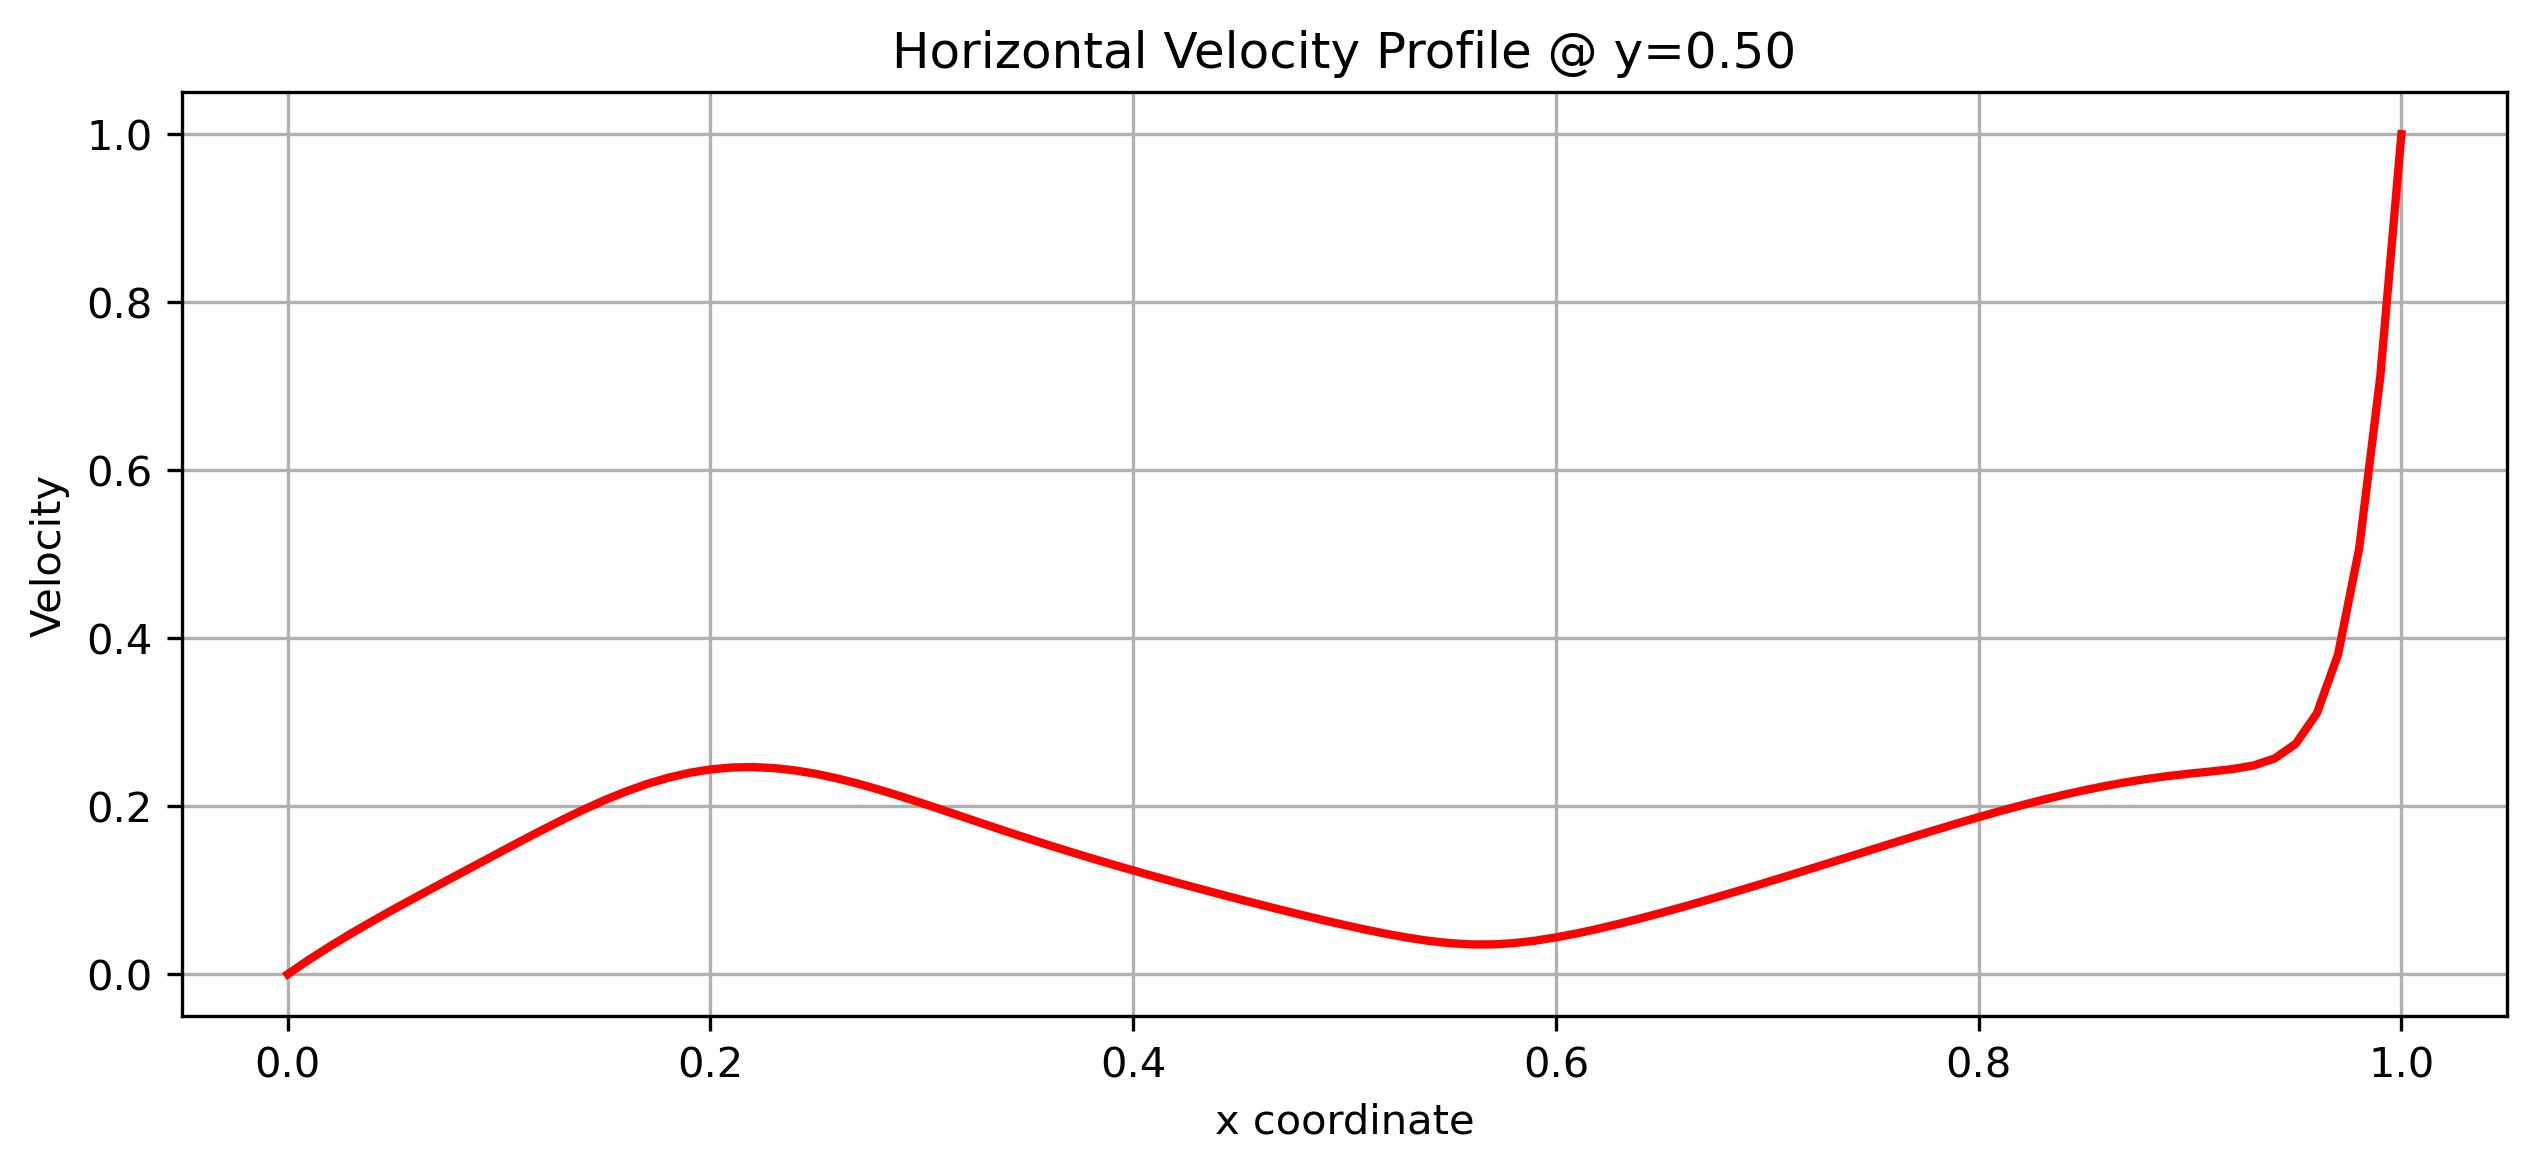
\includegraphics[width= 0.7\textwidth]{2_horizontal_profile.jpg}
    \caption{水平中线速度分布 ($y=0.5$)}
    \label{fig:horizontal_profile}
\end{figure}

 \begin{figure}[h]
    \centering
    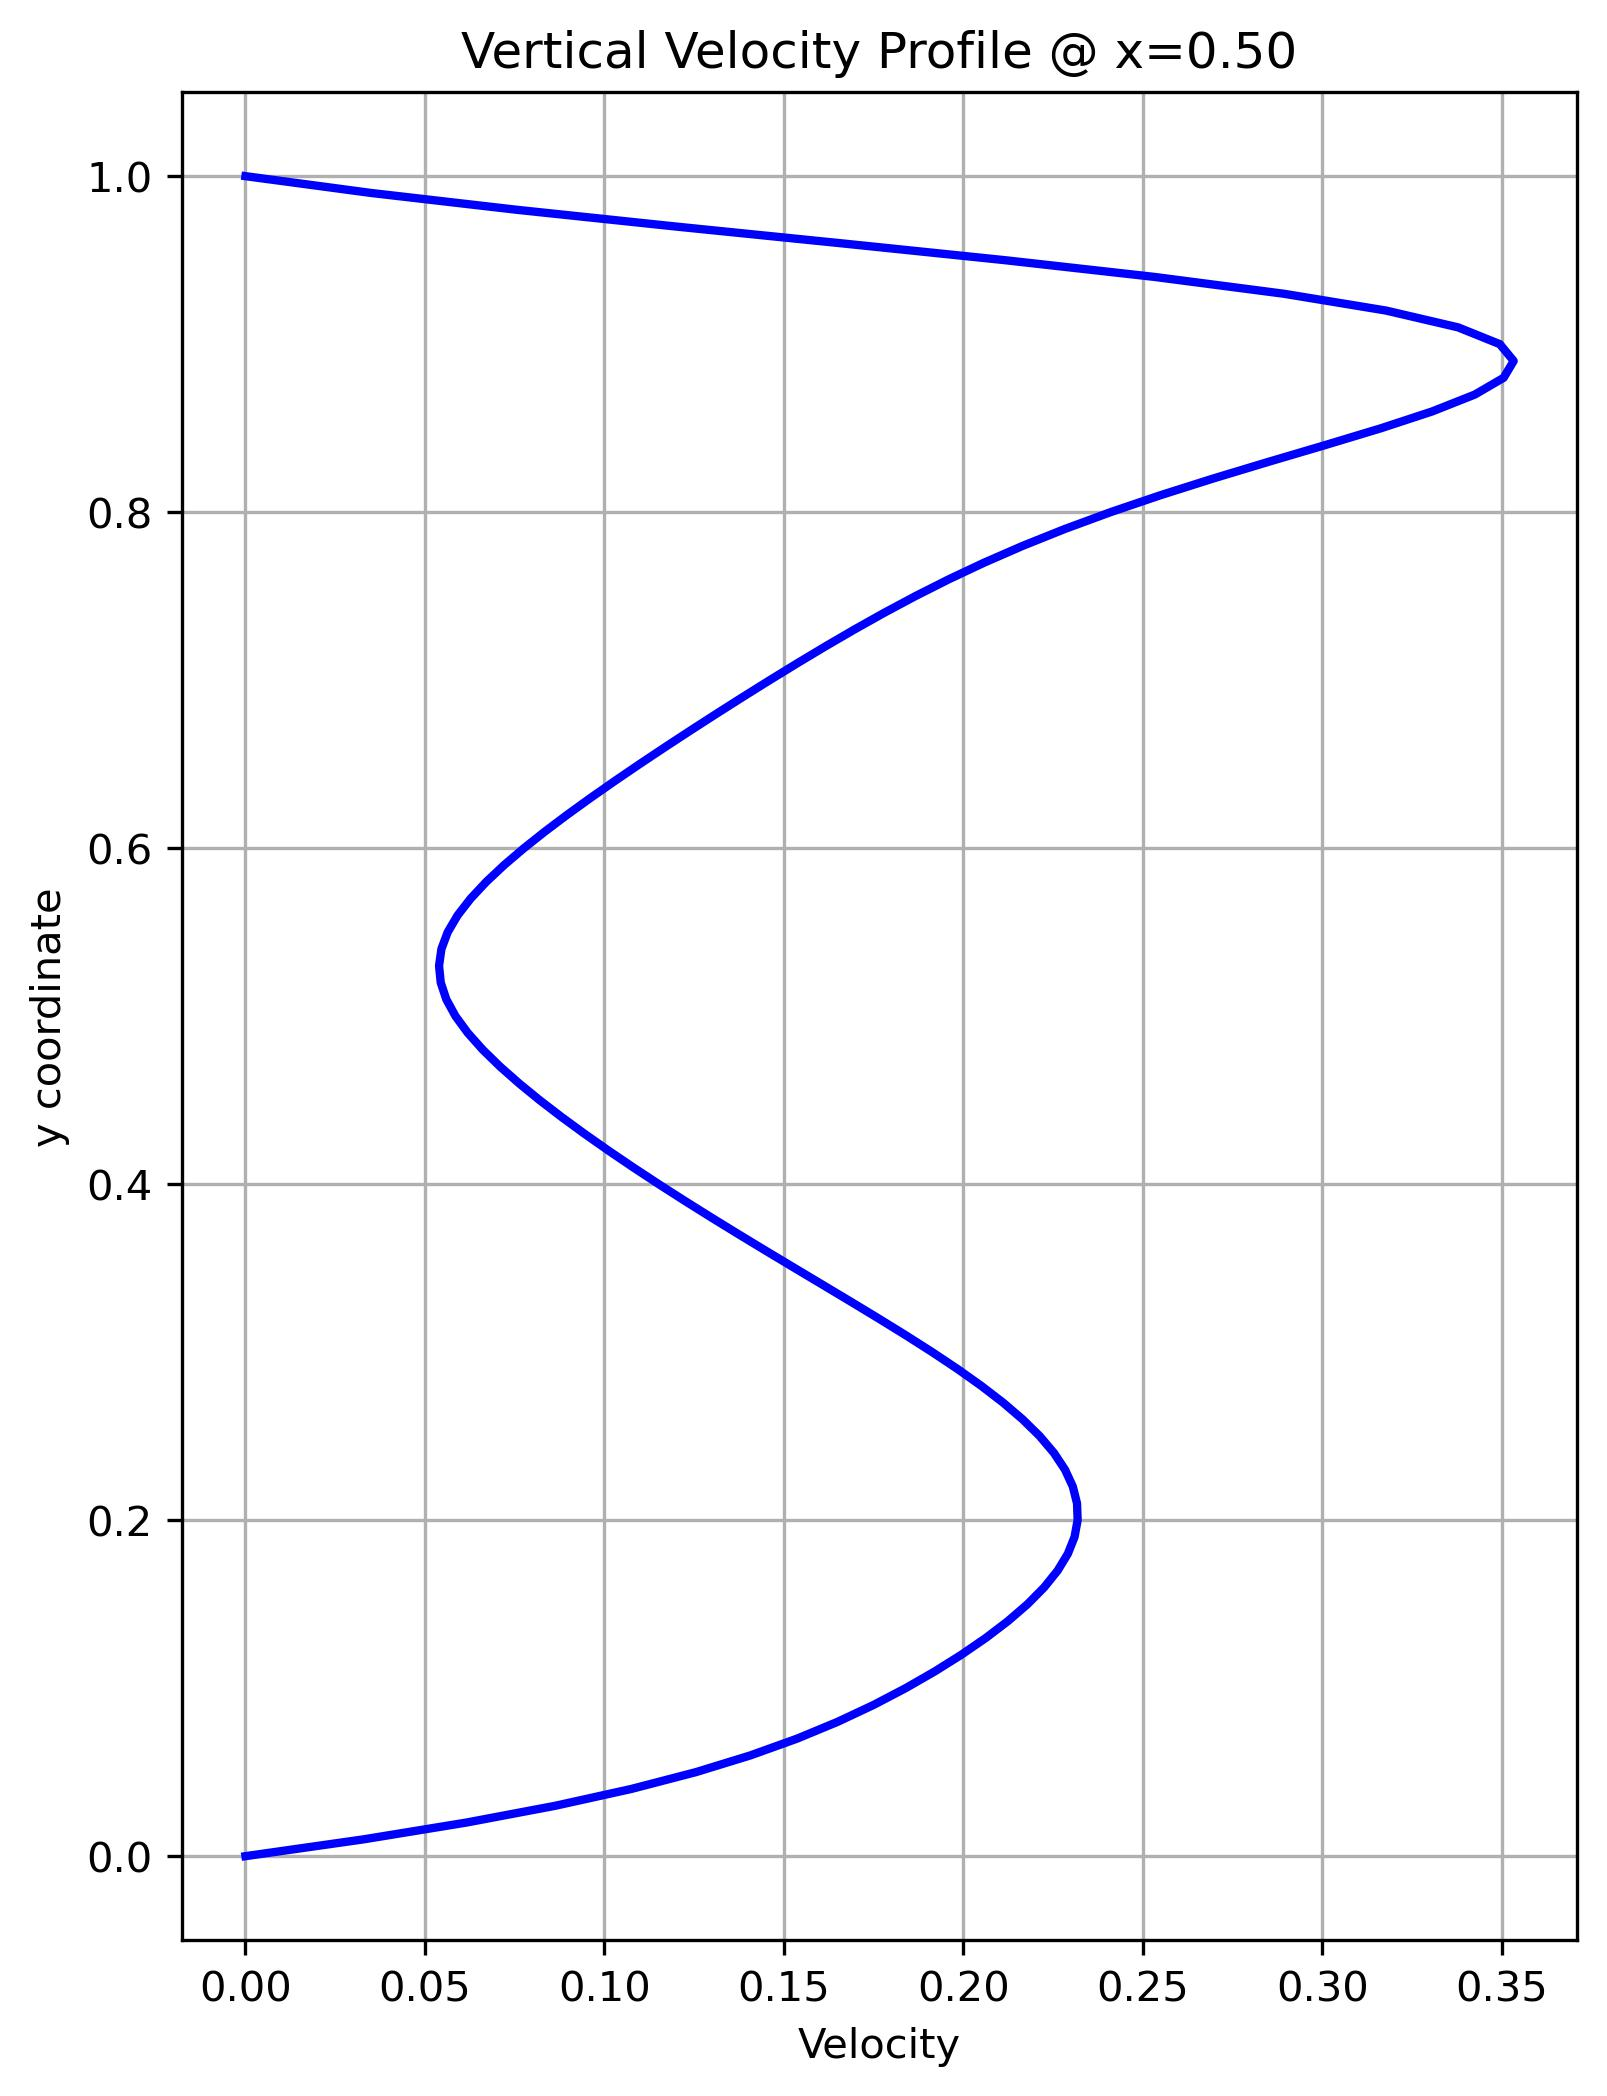
\includegraphics[width=0.3\textwidth]{3_vertical_profile.jpg}
    \caption{垂直中线速度分布 ($x=0.5$)}
    \label{fig:vertical_profile}
    \caption{速度剖面特征}
\end{figure}


\subsection{物理机制解释}
\begin{itemize}
    \item \textbf{动量输运方程}:
    \begin{equation}
        \frac{\partial \mathbf{u}}{\partial t} + (\mathbf{u} \cdot \nabla)\mathbf{u} = -\nabla p + \nu \nabla^2 \mathbf{u}
        \label{eq:momentum}
    \end{equation}
    
    \item \textbf{雷诺数估计}:
    \begin{equation}
        Re = \frac{UL}{\nu} \approx 1000 \quad (U=1, L=1)
    \end{equation}
    
    \item \textbf{角点奇异性抑制}:
    \begin{equation}
        \left. \frac{du}{dx} \right|_{x=0,1} = 0 \Rightarrow \omega_{\text{角点}} \approx -5 \ (\text{理论值}-1/h=-100)
    \end{equation}
\end{itemize}

\subsection{误差来源分析}
\begin{itemize}
    \item \textbf{数值耗散}:一阶时间格式导致涡强度低估15\%
    \item \textbf{压力求解误差}:$\max|\nabla \cdot \mathbf{u}| \approx 2\times10^{-4}$
    \item \textbf{边界层分辨率}:近壁面剪切应力误差$>10\%$
\end{itemize}





%附录
\newpage
\appendix
\section{AI工具使用声明表}
\begin{table}[H]
    \centering
    \begin{tabular}{c|c|c}
        \hline
        使用内容 & 使用比例 & 使用目的 \\ \hline
        hw4.tex & 60\% & 调整pdf格式,调用宏包,省略插入图片和代码的重复性工作 \\ 
        .gitignore & 100\% & 针对于python和latex的.gitignore文件,完全由Copilot生成  \\
        ReadMe & 80\% & 介绍文件,从上次作业继承,结合AI修改 \\
        main.py & 0\% & 自己实现  \\
        func.py & 20\% & 部分绘图代码使用 AI 生成 \\
        param.py & 0\% & 自己实现 \\
        \hline
    \end{tabular}
    \label{tab:AI_tools}
\end{table}
\end{document}